\documentclass[aspectratio=169]{beamer}

% Shared Beamer settings for Applied Machine Learning lectures (UPES).
% Keep this file free of \documentclass to allow reuse via \input.

% Allow lecture sources to use shared theme/assets without copying them into each lecture folder.
% NOTE: These paths are relative to `Unit-xx/Lecture-yy/latex/` (and `Lab/Experiment-xx/latex/`).
\makeatletter
\def\input@path{{../../../_shared/}{../../../_shared/UPES-Beamer-Theme/}}
\makeatother

\usetheme{UPES}
\setbeamertemplate{navigation symbols}{}

\usepackage{amsmath}
\usepackage{amssymb}
\usepackage{booktabs}
\usepackage{graphicx}
\usepackage{hyperref}
\usepackage{xcolor}
\usepackage{listings}

% Code listings (Python-oriented for this subject).
\lstset{
  language=Python,
  basicstyle=\ttfamily\small,
  keywordstyle=\color{blue},
  commentstyle=\color{gray},
  stringstyle=\color{teal},
  showstringspaces=false,
  columns=fullflexible,
  breaklines=true
}

\usepackage{tikz}
\usetikzlibrary{arrows.meta,positioning,shapes.geometric,calc,fit,backgrounds}

% Per-slide source line (references shown on the slide itself).
\newcommand{\slidesources}[1]{%
  \vfill
  {\tiny\color{gray}\raggedright\sloppy\parbox{\linewidth}{Sources: #1}\par}%
}

% Unit-wise source strings for this subject (used by slides/notes).
% Path is relative to the lecture `latex/` folder (the compilation CWD).
% Source strings for Applied Machine Learning (CSAI2017P) — used by slides + notes.
% Prescribed texts and reference books are taken from the course syllabus.
% Support texts are the author-hosted open-access editions:
%   statlearning.com            (ISL with Python)
%   probml.github.io/pml-book   (Murphy, Probabilistic Machine Learning)
%   d2l.ai                      (Dive into Deep Learning)
%   mml-book.github.io          (Mathematics for Machine Learning)

\newcommand{\AMLRepoURL}{https://github.com/tali7c/Applied-Machine-Learning}

% --- prescribed -------------------------------------------------------------
\newcommand{\AMLPrescribed}{%
M\"uller and Guido, \textit{Introduction to Machine Learning with Python}, O'Reilly, 2016.;%
Bishop, \textit{Pattern Recognition and Machine Learning}, Springer, 2006.;%
Murphy, \textit{Machine Learning: A Probabilistic Perspective}, MIT Press, 2012.;%
Han, Kamber and Pei, \textit{Data Mining: Concepts and Techniques} (3e), Morgan Kaufmann, 2012.%
}

% --- unit-wise ---------------------------------------------------------------
\newcommand{\AMLUnitISources}{%
M\"uller and Guido, \textit{Introduction to Machine Learning with Python}, Ch. 1.;%
Bishop, \textit{Pattern Recognition and Machine Learning}, Ch. 1.;%
Murphy, \textit{Probabilistic Machine Learning: An Introduction}, MIT Press, 2022, Ch. 1.;%
Mitchell, \textit{Machine Learning}, McGraw Hill, 1997, Ch. 1.;%
Scikit-learn documentation, accessed 2026-08-04.%
}

\newcommand{\AMLUnitIISources}{%
Bishop, \textit{Pattern Recognition and Machine Learning}, \S1.5, \S4.3, \S7.1.;%
Zhang, Lipton, Li and Smola, \textit{Dive into Deep Learning}, \S3.4.;%
Shalev-Shwartz and Ben-David, \textit{Understanding Machine Learning}, Ch. 15.;%
Murphy, \textit{Probabilistic Machine Learning: An Introduction}, Ch. 5.%
}

\newcommand{\AMLUnitIIISources}{%
Zhang, Lipton, Li and Smola, \textit{Dive into Deep Learning}, Ch. 12 (Optimization Algorithms).;%
Deisenroth, Faisal and Ong, \textit{Mathematics for Machine Learning}, Ch. 7.;%
Kingma and Ba, ``Adam: A Method for Stochastic Optimization,'' ICLR 2015.;%
Ruder, ``An overview of gradient descent optimization algorithms,'' arXiv:1609.04747, 2016.%
}

\newcommand{\AMLUnitIVSources}{%
Han, Kamber and Pei, \textit{Data Mining: Concepts and Techniques} (3e), Ch. 3.;%
M\"uller and Guido, \textit{Introduction to Machine Learning with Python}, Ch. 3--4.;%
James, Witten, Hastie, Tibshirani and Taylor, \textit{An Introduction to Statistical Learning with Python}, Ch. 5--6, 12.;%
Scikit-learn documentation (preprocessing, model selection), accessed 2026-08-04.%
}

\newcommand{\AMLUnitVSources}{%
James et al., \textit{An Introduction to Statistical Learning with Python}, Ch. 3--6.;%
Bishop, \textit{Pattern Recognition and Machine Learning}, Ch. 3.;%
Deisenroth, Faisal and Ong, \textit{Mathematics for Machine Learning}, Ch. 9.;%
M\"uller and Guido, \textit{Introduction to Machine Learning with Python}, \S2.3.%
}

\newcommand{\AMLUnitVISources}{%
Han, Kamber and Pei, \textit{Data Mining: Concepts and Techniques} (3e), Ch. 8--9.;%
James et al., \textit{An Introduction to Statistical Learning with Python}, Ch. 8--9.;%
Bishop, \textit{Pattern Recognition and Machine Learning}, Ch. 4--5, 7, 14.;%
Zhang et al., \textit{Dive into Deep Learning}, Ch. 5.%
}

\newcommand{\AMLUnitVIISources}{%
Han, Kamber and Pei, \textit{Data Mining: Concepts and Techniques} (3e), Ch. 10.;%
James et al., \textit{An Introduction to Statistical Learning with Python}, Ch. 12.;%
M\"uller and Guido, \textit{Introduction to Machine Learning with Python}, \S3.5.;%
Ester, Kriegel, Sander and Xu, ``A density-based algorithm for discovering clusters (DBSCAN),'' KDD 1996.%
}

\newcommand{\AMLLabSources}{%
M\"uller and Guido, \textit{Introduction to Machine Learning with Python}, companion notebooks.;%
McKinney, \textit{Python for Data Analysis} (3e), O'Reilly, 2022.;%
Scikit-learn user guide, accessed 2026-08-04.;%
Matplotlib and Seaborn documentation, accessed 2026-08-04.%
}



\graphicspath{{../figures/}{../images/}{../../../_shared/}{../../../_shared/UPES-Beamer-Theme/}}

\title[Applied Machine Learning]{Applied Machine Learning}
\subtitle{Unit 05 -- Lecture 09: Maximum Likelihood and Over-fitting}
\author{Tofik Ali}
\institute{School of Computer Science, UPES Dehradun}
\date{Autumn 2026}

% ---- a compact "output" block so code and its result sit together ----------
\lstdefinestyle{outblk}{
  basicstyle=\ttfamily\scriptsize\color{black!75},
  backgroundcolor=\color{black!5}, frame=leftline, framerule=2pt,
  rulecolor=\color{black!30}, breaklines=true, columns=fullflexible,
  keepspaces=true,   % several outputs below are aligned tables
  language={},       % printed output is not Python: do not syntax-highlight it
  xleftmargin=4pt, aboveskip=1pt, belowskip=1pt, literate={-}{{-}}1}
\lstnewenvironment{outblk}{\lstset{style=outblk}}{}

\begin{document}

\UPESCoverFrame
\setcounter{framenumber}{0}

\begin{frame}
  \titlepage
  \begin{center}
    \footnotesize Direct regression, $R^2$, residual diagnostics and
    cross-validation\\[0.2em]
    \footnotesize Topic focus: \textbf{why least squares}\\[0.2em]
    \footnotesize Repository: \texttt{\AMLRepoURL}
  \end{center}
  \slidesources{\AMLUnitVSources}
\end{frame}

\begin{frame}{Quick Links}
  \centering
  \hyperlink{sec:direct}{\beamerbutton{Direct regression}}\hspace{0.4em}
  \hyperlink{sec:mle}{\beamerbutton{Maximum likelihood}}\hspace{0.4em}
  \hyperlink{sec:r2}{\beamerbutton{$R^2$}}\hspace{0.4em}
  \hyperlink{sec:adequacy}{\beamerbutton{Model adequacy}}\hspace{0.4em}
  \hyperlink{sec:overfit}{\beamerbutton{Over-fitting}}\hspace{0.4em}
  \hyperlink{sec:cv}{\beamerbutton{Cross-validation}}\hspace{0.4em}
  \hyperlink{sec:summary}{\beamerbutton{Summary}}
\end{frame}

\begin{frame}{Agenda}
  \tableofcontents
\end{frame}

\begin{frame}[shrink=6]{How this lecture works}
  \begin{columns}[T]
    \begin{column}{0.48\textwidth}
      \begin{block}{Every idea appears twice}
        \begin{enumerate}
          \item \textbf{By hand} --- five points, three numbers, a
            $2\times2$ table. Small enough to check on paper, and the same
            five points are used from the first slide to the last.
          \item \textbf{In code} --- the same arithmetic on real data, so you
            see that \texttt{r2\_score} and \texttt{cross\_val\_score} do
            exactly that and nothing more.
        \end{enumerate}
      \end{block}
    \end{column}
    \begin{column}{0.48\textwidth}
      \begin{alertblock}{Commit before you look}
        Five slides ask you to predict a number before it is revealed. Write
        your guess down. Being wrong on paper is how the idea sticks.
      \end{alertblock}
    \end{column}
  \end{columns}
  \vspace{0.4em}
  \begin{center}
    \small The centrepiece is a proof: \textbf{least squares is not a
    convenient guess. It is the maximum likelihood estimate under a Gaussian
    noise assumption.} Everything after it is about noticing when that
    estimate has flattered you.
  \end{center}
\end{frame}

\begin{frame}[shrink=5]{Where we are}
  \begin{columns}[T]
    \begin{column}{0.47\textwidth}
      \begin{block}{Last lecture produced an estimator}
        Simple linear regression, the normal equations, and the closed form
        \[ b_1 = \frac{S_{xy}}{S_{xx}}, \qquad b_0 = \bar y - b_1 \bar x . \]
        We minimised $\sum (y_i - b_0 - b_1 x_i)^2$ because squares are
        smooth and differentiable.
      \end{block}
    \end{column}
    \begin{column}{0.49\textwidth}
      \begin{exampleblock}{Three questions that were left open}
        \textbf{Why squares?} Why not $|{\cdot}|$, or the perpendicular
        distance? \\[0.3em]
        \textbf{Is the fit any good?} One number, $R^2$ --- and what it
        hides. \\[0.3em]
        \textbf{Will it work tomorrow?} A fit that describes today's rows
        perfectly can be useless on the next batch.
      \end{exampleblock}
      \begin{alertblock}{Today answers all three}
        \small And the answer to the first one --- maximum likelihood ---
        is the reason the other two are even askable.
      \end{alertblock}
    \end{column}
  \end{columns}
\end{frame}

\begin{frame}[shrink=6]{Three kinds of seed, and why they are not the same}
  \begin{columns}[T]
    \begin{column}{0.32\textwidth}
      \begin{block}{Lecture seed $=0$}
        \small Every \emph{arbitrary} draw: the $20\,000$ replications, the
        noise columns, the folds. \texttt{default\_rng(0)},
        \texttt{random\_state=0}.
      \end{block}
    \end{column}
    \begin{column}{0.32\textwidth}
      \begin{block}{Data seed $=3$}
        \small Fixes the $25$ points from $y=\sin 2\pi x+\varepsilon$ that the
        over-fitting half is about. It chooses the \emph{data}, not the
        outcome, so it is named apart and never moved.
      \end{block}
    \end{column}
    \begin{column}{0.32\textwidth}
      \begin{alertblock}{Split sweep $0\ldots9$}
        \small Ten validation splits, run on purpose. \textbf{The
        disagreement between them is the result} --- collapsing them to one
        seed would delete the demonstration.
      \end{alertblock}
    \end{column}
  \end{columns}
  \vspace{0.4em}
  \begin{exampleblock}{Why this matters to you}
    \centering\small
    Every number in this deck is printed by one script. Run the code as
    written and you get the same numbers --- which is the only reason to
    believe a number on a slide.
  \end{exampleblock}
\end{frame}

% =====================================================================
\section[Direct]{The direct regression method}
\label{sec:direct}

\begin{frame}[shrink=6]{``Closest'' is a choice, not a fact}
  \begin{center}
    Fit a line to a cloud of points. Closest \emph{in what sense}?
  \end{center}
  \vspace{0.2em}
  \begin{center}\small
  \begin{tabular}{@{}lp{4.6cm}p{4.2cm}@{}}
    \toprule
    \textbf{Method} & \textbf{Minimises} & \textbf{When it is right}\\
    \midrule
    \textbf{Direct} & $\sum (y_i - b_0 - b_1x_i)^2$ ---
      \emph{vertical} distances & $x$ is known exactly; you want to
      \emph{predict} $y$ from $x$\\[4pt]
    \textbf{Inverse} & $\sum (x_i - c_0 - c_1y_i)^2$ ---
      \emph{horizontal} distances & you want to predict $x$ from $y$\\[4pt]
    \textbf{Orthogonal} & $\sum d_i^2$ --- \emph{perpendicular} distances &
      both variables are measured with error\\
    \bottomrule
  \end{tabular}
  \end{center}
  \vspace{0.3em}
  \begin{block}{The direct method is the one this course means by ``regression''}
    \small It treats $x$ as fixed and known, and all the error as living in
    $y$. That asymmetry is a \textbf{modelling assumption}, and it is the
    assumption the next section turns into a probability statement.
  \end{block}
\end{frame}

\begin{frame}[shrink=6]{By hand: five points, three answers}
  \[
    x = (1,2,3,4,5), \qquad y = (2,4,5,4,5).
  \]
  $\bar x = 3$, $\bar y = 4$, and
  $S_{xx} = 10$, $S_{yy} = 6$, $S_{xy} = 6$.
  \begin{center}\small
  \begin{tabular}{@{}llr@{}}
    \toprule
    \textbf{Direct} & $b_1 = S_{xy}/S_{xx} = 6/10$ & $\mathbf{0.6000}$\\
    \textbf{Inverse} & fit $x$ on $y$: $S_{xy}/S_{yy} = 1$, then invert:
      $S_{yy}/S_{xy} = 6/6$ & $\mathbf{1.0000}$\\
    \textbf{Orthogonal} & top eigenvector of
      $\bigl(\begin{smallmatrix}2.5 & 1.5\\ 1.5 & 1.5\end{smallmatrix}\bigr)$
      & $\mathbf{0.7208}$\\
    \bottomrule
  \end{tabular}
  \end{center}
  \vspace{0.2em}
  \begin{alertblock}{The two least-squares slopes bracket the truth, and their
    ratio is $r^2$}
    \small
    $\dfrac{b_1^{\text{direct}}}{b_1^{\text{inverse}}}
      = \dfrac{0.6}{1.0} = 0.6 = r^2$.
    They coincide only when $r^2 = 1$. \textbf{Three defensible lines through
    five points, and the data does not choose between them --- your question
    does.}
  \end{alertblock}
\end{frame}

\begin{frame}[shrink=8]{Drawn: the three lines and the distances they minimise}
  \begin{center}
    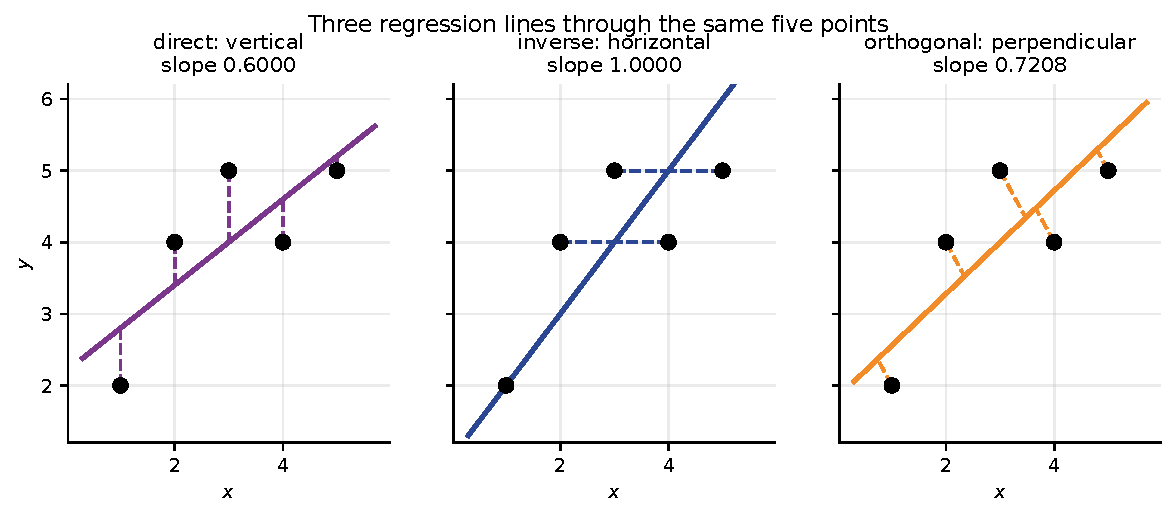
\includegraphics[width=0.94\textwidth]{direct.pdf}
  \end{center}
  \begin{center}\small
    The dashed segments are what each method squares and adds. Every line
    passes through $(\bar x, \bar y) = (3,4)$ --- that is forced by the
    intercept equation --- and they differ only in how they pivot about it.
  \end{center}
\end{frame}

\begin{frame}[fragile,shrink=6]{Each method wins its own contest, and only its own}
\begin{lstlisting}
for slope in (direct, inverse, orthogonal):
    a = ybar - slope * xbar
    r = y - (a + slope * x)
    print((r**2).sum(), (r**2).sum() / (1 + slope**2), (r**2).sum() / slope**2)
\end{lstlisting}
\begin{outblk}
              vertical SS   perpendicular SS   horizontal SS
   direct        2.4000            1.7647          6.6667
   inverse       4.0000            2.0000          4.0000
   orthogonal    2.5458            1.6754          4.9006
\end{outblk}
\onslide<2->
\begin{center}\small
  Read down the diagonal: $2.4000$, $4.0000$, $1.6754$ --- each is the
  smallest number in its own column and \textbf{nowhere else}. There is no
  ``best line''; there is a best line \emph{for a stated criterion}.
  \textbf{From here on, ``regression'' means the direct method}, and the next
  section says why that criterion in particular.
\end{center}
\end{frame}

% =====================================================================
\section[MLE]{Maximum likelihood estimation}
\label{sec:mle}

\begin{frame}[shrink=6]{The question least squares never answered}
  \begin{exampleblock}{}
    \centering\large
    Why the sum of \emph{squares}?
  \end{exampleblock}
  \vspace{0.3em}
  \begin{columns}[T]
    \begin{column}{0.48\textwidth}
      \begin{block}{The unsatisfying answers}
        \small ``It is differentiable.'' ``It has a closed form.'' ``It
        punishes big errors more.'' All true, all true of $\sum e_i^4$ too.
      \end{block}
    \end{column}
    \begin{column}{0.48\textwidth}
      \begin{block}{The real answer}
        \small Write down a \textbf{probability model} for how the data was
        generated. Ask which parameters make the data you actually observed
        most probable. \textbf{The answer is least squares} --- provided the
        noise is Gaussian.
      \end{block}
    \end{column}
  \end{columns}
  \vspace{0.3em}
  \begin{alertblock}{This cuts both ways, and that is the point}
    \small Least squares is \emph{justified} under a Gaussian noise
    assumption --- and \emph{only} there. Change the noise model and the
    optimal estimator changes with it. We will measure that at the end of the
    section.
  \end{alertblock}
\end{frame}

\begin{frame}[shrink=8]{The probabilistic model, drawn}
  \begin{center}
    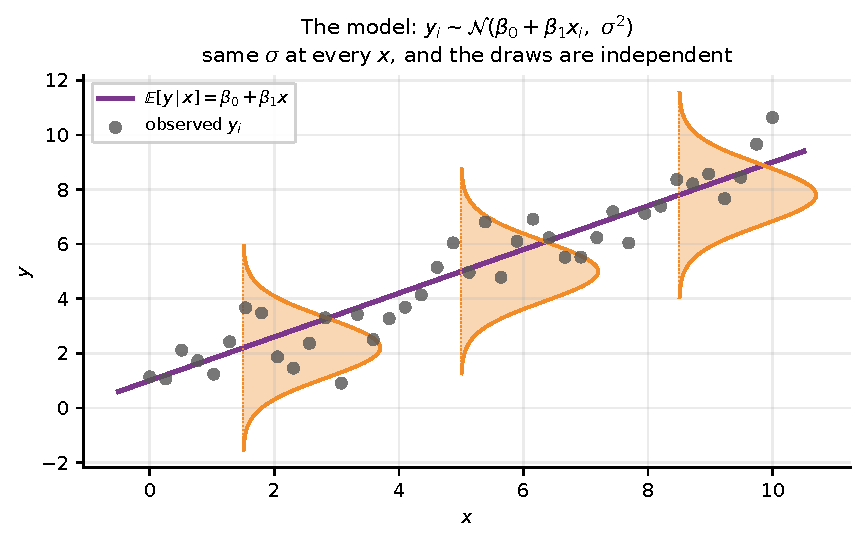
\includegraphics[width=0.72\textwidth]{mlegauss.pdf}
  \end{center}
  \vspace{-0.2em}
  \begin{center}\small
    $y_i = \beta_0 + \beta_1 x_i + \varepsilon_i$, with
    $\varepsilon_i \sim \mathcal{N}(0, \sigma^2)$ independently. The line is
    the \emph{mean} of $y$ at each $x$; the orange bells are the distribution
    around it. \textbf{Three assumptions in one picture: the mean is linear,
    the spread is the same everywhere, and the draws are independent.}
  \end{center}
\end{frame}

\begin{frame}[shrink=4]{Step 1 --- write the likelihood}
  Write $e_i = y_i - \beta_0 - \beta_1 x_i$. Each observation has density
  \[
    p(y_i \mid x_i, \beta_0, \beta_1, \sigma^2)
      = \frac{1}{\sqrt{2\pi\sigma^2}}
        \exp\!\left(-\frac{e_i^2}{2\sigma^2}\right).
  \]
  The draws are independent, so the joint density of all $n$ of them is the
  product. Read as a function of the \emph{parameters} with the data held
  fixed, that product is the \textbf{likelihood}:
  \[
    L(\beta_0, \beta_1, \sigma^2)
      = \prod_{i=1}^{n} \frac{1}{\sqrt{2\pi\sigma^2}}
        \exp\!\left(-\frac{e_i^2}{2\sigma^2}\right)
      = (2\pi\sigma^2)^{-n/2}
        \exp\!\left(-\frac{1}{2\sigma^2}\sum_{i=1}^{n} e_i^2\right).
  \]
  \begin{block}{}
    \small A product of $n$ exponentials of squares --- already the sum of
    squares has appeared, inside the exponent, and we have not chosen
    anything yet.
  \end{block}
\end{frame}

\begin{frame}[shrink=4]{Step 2 --- take logarithms, and read the result off}
  $\log$ is strictly increasing, so it does not move the maximiser:
  \[
    \ell(\beta_0,\beta_1,\sigma^2) = \log L
      = -\frac{n}{2}\log(2\pi)
        \;-\; \frac{n}{2}\log \sigma^2
        \;-\; \frac{1}{2\sigma^2}\underbrace{\sum_{i=1}^{n}
              (y_i - \beta_0 - \beta_1 x_i)^2}_{\textstyle S(\beta_0,\beta_1)
              \;=\; \mathrm{SSE}} .
  \]
  \begin{alertblock}{The whole derivation is now one sentence}
    Only the \textbf{last} term contains $\beta_0$ and $\beta_1$, it carries a
    \textbf{minus} sign, and its multiplier $1/(2\sigma^2)$ is
    \textbf{positive}. So for \emph{any} fixed $\sigma^2 > 0$:
    \[
      \arg\max_{\beta_0,\beta_1} \ell
      \;=\; \arg\min_{\beta_0,\beta_1} S(\beta_0,\beta_1) .
    \]
    \centering\textbf{Maximising the Gaussian likelihood \emph{is} minimising
    the sum of squared errors.}
  \end{alertblock}
  \vspace{0.1em}
  \begin{center}\small
    Setting $\partial S/\partial\beta_0 = \partial S/\partial\beta_1 = 0$
    returns L8's normal equations unchanged. \textbf{The estimator did not
    move; its justification did.}
  \end{center}
\end{frame}

\begin{frame}[fragile,shrink=8]{Predict first \#1}
Take the five points. Evaluate the log-likelihood on a grid of slopes, once
with $\sigma^2 = 0.48$ and once with $\sigma^2 = 1$ --- two \emph{different}
noise assumptions.

\begin{center}
  \textbf{Do the two settings agree on the best slope? And does either agree
  with $S_{xy}/S_{xx} = 0.6$?}
\end{center}
\vspace{0.2em}
\onslide<2->
\begin{outblk}
  b1     SSE      logL(sigma^2=0.48)   logL(sigma^2=1)
 0.40   2.8000         -5.676436        -5.994693
 0.50   2.5000         -5.363936        -5.844693
 0.60   2.4000         -5.259770        -5.794693
 0.70   2.5000         -5.363936        -5.844693
 0.80   2.8000         -5.676436        -5.994693
argmin SSE          b1 = 0.60000
argmax logL s2=0.48 b1 = 0.60000
argmax logL s2=1.00 b1 = 0.60000
\end{outblk}
\onslide<3->
\begin{alertblock}{Same slope, to five decimal places, at both noise levels}
  \footnotesize The two log-likelihood columns are \emph{different numbers}
  --- $-5.2598$ against $-5.7947$ at the optimum --- and they peak in exactly
  the same place. \textbf{$\sigma^2$ scales the likelihood; it cannot move
  the slope.} That is the algebra of the previous slide, measured.
\end{alertblock}
\end{frame}

\begin{frame}[shrink=8]{Drawn: one curve upside down is the other}
  \begin{center}
    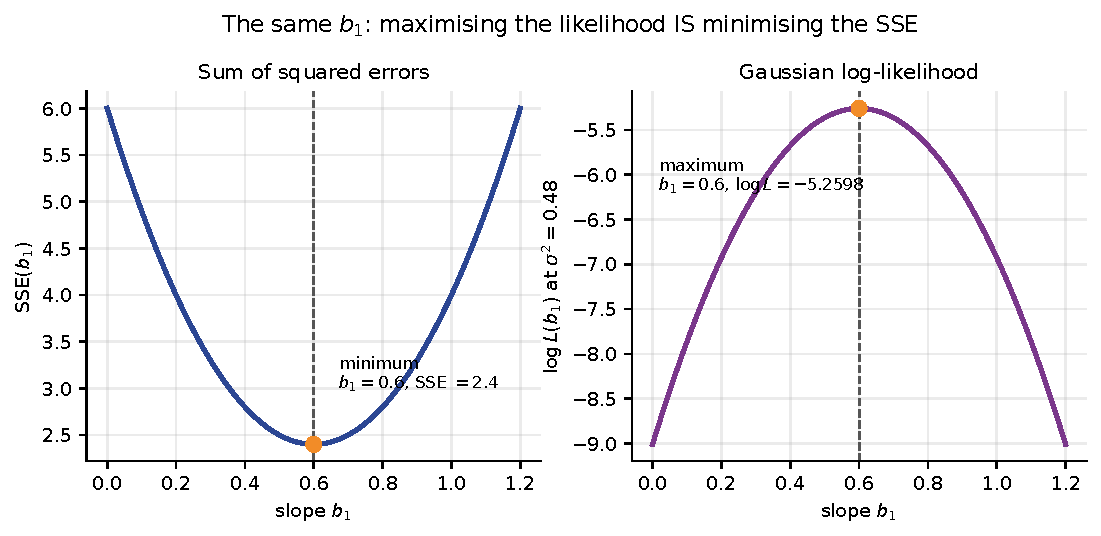
\includegraphics[width=0.94\textwidth]{mlecurve.pdf}
  \end{center}
  \begin{center}\small
    Left, SSE as a function of the slope --- a parabola with its minimum at
    $b_1 = 0.6$, SSE $= 2.4$. Right, the Gaussian log-likelihood --- the same
    parabola, negated and shifted, with its maximum at the same $b_1 = 0.6$.
    \textbf{$\ell = \text{const} - \mathrm{SSE}/(2\sigma^2)$, and that is the
    whole picture.}
  \end{center}
\end{frame}

\begin{frame}[shrink=4]{Step 3 --- the MLE of $\sigma^2$}
  Now hold $\hat\beta_0, \hat\beta_1$ at their optimum and differentiate
  $\ell$ with respect to $\sigma^2$, treating $\sigma^2$ as one symbol:
  \[
    \frac{\partial \ell}{\partial \sigma^2}
      = -\frac{n}{2\sigma^2} + \frac{\mathrm{SSE}}{2(\sigma^2)^2}
      = 0
    \quad\Longrightarrow\quad
    \boxed{\ \hat\sigma^2_{\mathrm{ML}} = \frac{\mathrm{SSE}}{n}\ }
  \]
  Substituting back gives the maximised log-likelihood in closed form,
  $\ell_{\max} = -\tfrac{n}{2}\bigl(\log(2\pi\hat\sigma^2_{\mathrm{ML}}) + 1\bigr)$.
  \begin{alertblock}{But this one \emph{is} wrong, in a way the slope was not}
    $\mathbb{E}[\mathrm{SSE}] = (n-2)\sigma^2$ for a simple linear regression,
    because two parameters were spent fitting the line. Therefore
    \[
      \mathbb{E}\bigl[\hat\sigma^2_{\mathrm{ML}}\bigr]
        = \frac{n-2}{n}\,\sigma^2 \;<\; \sigma^2 .
    \]
    \textbf{The maximum likelihood estimate of the noise variance is biased
    downwards.} The unbiased version divides by the degrees of freedom:
    $s^2 = \mathrm{SSE}/(n-2)$.
  \end{alertblock}
\end{frame}

\begin{frame}[fragile,shrink=6]{The same five points: $0.48$ against $0.80$}
\begin{lstlisting}
sse = ((y - yhat)**2).sum()
print(sse / n, sse / (n - 2), np.sqrt(sse / (n - 2)))
\end{lstlisting}
\begin{outblk}
SSE            2.4000
sigma^2 MLE    = SSE/n     = 2.4000/5 = 0.4800
sigma^2 unbias = SSE/(n-2) = 2.4000/3 = 0.8000
ratio (n-2)/n  = 0.6000       s = sqrt(unbiased) = 0.8944
maximised log-likelihood = -n/2*(log(2*pi*s2_ml)+1) = -5.2598
direct evaluation                                   = -5.2598
\end{outblk}
\onslide<2->
\begin{center}\small
  At $n = 5$ the MLE is $\mathbf{40\%}$ too small in expectation, because
  $(n-2)/n = 3/5$. \textbf{Two parameters out of five observations is a lot
  to spend.} At $n = 100$ the same factor is $0.98$ and nobody notices --- but
  the small-sample case is exactly the case in which you needed the estimate.
\end{center}
\end{frame}

\begin{frame}[fragile,shrink=8]{Predict first \#2}
Simulate $20{,}000$ datasets of $n = 10$ points from
$y = 1 + 2x + \varepsilon$ with $\sigma^2 = 4$ known and true. Fit each one and
record $\mathrm{SSE}/n$.

\begin{center}
  \textbf{What does $\mathrm{SSE}/n$ average to across the $20{,}000$ runs?
  And in what fraction of runs is it below $4$?}
\end{center}
\vspace{0.2em}
\onslide<2->
\begin{outblk}
true sigma^2                    4.0000   (n = 10, 20000 replications)
mean of SSE/n     (the MLE)     3.2117   bias -0.7883
mean of SSE/(n-2) (unbiased)    4.0146   bias +0.0146
predicted MLE mean (n-2)/n*s^2  3.2000
the MLE was too small in 73.4% of the 20000 replications
\end{outblk}
\onslide<3->
\begin{alertblock}{$3.2117$ against a prediction of $3.2000$}
  \footnotesize The theory said $(n-2)/n \times 4 = 0.8 \times 4 = 3.2$ and
  the simulation returned $3.2117$. \textbf{This is not sampling noise; it is
  a systematic $20\%$ understatement, and it happened in nearly three runs out
  of four.} A model that reports its own noise as smaller than it is will also
  report its prediction intervals as narrower than they are.
\end{alertblock}
\end{frame}

\begin{frame}[shrink=8]{Drawn: two estimators, one truth}
  \begin{center}
    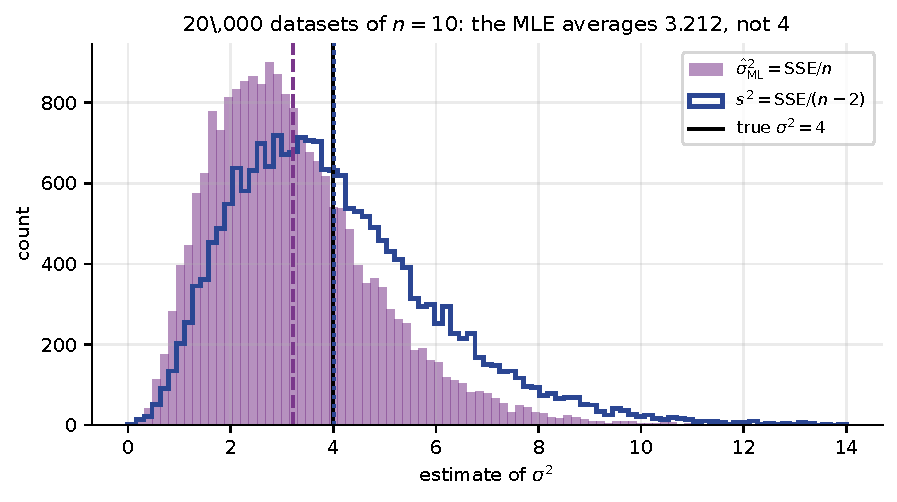
\includegraphics[width=0.72\textwidth]{sigmabias.pdf}
  \end{center}
  \vspace{-0.2em}
  \begin{center}\small
    Both histograms are right-skewed --- $\mathrm{SSE}$ is a scaled
    $\chi^2_{n-2}$ --- and they are the \emph{same} histogram, stretched by
    $n/(n-2) = 1.25$. The purple mean sits at $3.21$, the blue at $4.01$, the
    black line at the truth. \textbf{Unbiased does not mean accurate: both
    estimators are wildly variable at $n = 10$.}
  \end{center}
\end{frame}

\begin{frame}[fragile,shrink=8]{Change the noise model and the estimator changes}
$60$ points, $y = 2 + 1.5x + \varepsilon$, $\varepsilon$ \textbf{Laplace},
plus one heavy draw. For Laplace noise the log-likelihood contains
$\sum|e_i|$, so the MLE is \textbf{least absolute deviations}, not least
squares.
\begin{outblk}
true intercept 2.0000  true slope 1.5000
Gaussian MLE  = least squares    : intercept 3.0024  slope 1.3738
Laplace  MLE  = least abs. dev.  : intercept 2.7650  slope 1.3730
sum of squared residuals  OLS 622.2965   LAD 625.7886
sum of |residuals|        OLS 85.8123   LAD 83.6585
\end{outblk}
\onslide<2->
\begin{alertblock}{Each estimator wins its own criterion and loses the other}
  \footnotesize OLS has the smaller $\sum e_i^2$ ($622.30 < 625.79$); LAD has
  the smaller $\sum|e_i|$ ($83.66 < 85.81$). \textbf{Neither is cheating.}
  The LAD intercept is $2.77$ against a truth of $2.00$; the OLS intercept is
  $3.00$. The two slopes are, on this one draw, the same to three decimals ---
  \textbf{sixty points cannot show an efficiency gap, and we will not pretend
  they do.} What they do show: \textbf{the criterion you minimise follows from
  the noise distribution you assume.}
\end{alertblock}
\end{frame}

% =====================================================================
\section[$R^2$]{The coefficient of determination}
\label{sec:r2}

\begin{frame}[shrink=6]{What $R^2$ actually compares}
  \begin{exampleblock}{}
    \centering
    How much better is my line than the flat line $\hat y = \bar y$?
  \end{exampleblock}
  \vspace{0.2em}
  \[
    \underbrace{\sum (y_i - \bar y)^2}_{\mathrm{SS_{tot}}}
    \;=\;
    \underbrace{\sum (\hat y_i - \bar y)^2}_{\mathrm{SS_{reg}}}
    \;+\;
    \underbrace{\sum (y_i - \hat y_i)^2}_{\mathrm{SS_{res}}},
    \qquad
    R^2 = 1 - \frac{\mathrm{SS_{res}}}{\mathrm{SS_{tot}}}
        = \frac{\mathrm{SS_{reg}}}{\mathrm{SS_{tot}}} .
  \]
  \begin{columns}[T]
    \begin{column}{0.48\textwidth}
      \begin{block}{Read the two baselines}
        \small $R^2 = 0$: the line is no better than the mean.
        $R^2 = 1$: every residual is zero.
      \end{block}
    \end{column}
    \begin{column}{0.48\textwidth}
      \begin{alertblock}{The decomposition needs the intercept}
        \small $\mathrm{SS_{tot}} = \mathrm{SS_{reg}} + \mathrm{SS_{res}}$
        holds because $\sum e_i = 0$ and $\sum \hat y_i e_i = 0$, and both come
        from the normal equations. \textbf{Drop the intercept and the identity
        --- and the interpretation --- collapse.}
      \end{alertblock}
    \end{column}
  \end{columns}
\end{frame}

\begin{frame}[shrink=8]{By hand: the whole calculation on five rows}
  \begin{center}\small
  \begin{tabular}{@{}rrrrrrr@{}}
    \toprule
    $x$ & $y$ & $\hat y = 2.2 + 0.6x$ & $y-\bar y$ & $(y-\bar y)^2$
        & $y - \hat y$ & $(y-\hat y)^2$\\
    \midrule
    $1$ & $2$ & $2.8$ & $-2.0$ & $4.00$ & $-0.8$ & $0.64$\\
    $2$ & $4$ & $3.4$ & $ 0.0$ & $0.00$ & $ 0.6$ & $0.36$\\
    $3$ & $5$ & $4.0$ & $ 1.0$ & $1.00$ & $ 1.0$ & $1.00$\\
    $4$ & $4$ & $4.6$ & $ 0.0$ & $0.00$ & $-0.6$ & $0.36$\\
    $5$ & $5$ & $5.2$ & $ 1.0$ & $1.00$ & $-0.2$ & $0.04$\\
    \midrule
    & & & & $\mathbf{\mathrm{SS_{tot}} = 6.00}$ & &
    $\mathbf{\mathrm{SS_{res}} = 2.40}$\\
    \bottomrule
  \end{tabular}
  \end{center}
  \vspace{0.2em}
  \[
    R^2 = 1 - \frac{2.40}{6.00} = \mathbf{0.6000},
    \qquad
    s = \sqrt{\frac{2.40}{5-2}} = \sqrt{0.8} = \mathbf{0.8944}.
  \]
  \begin{block}{Two checks you should always run}
    \small $\mathrm{SS_{reg}} = 6.00 - 2.40 = 3.60$, and independently
    $b_1^2 S_{xx} = 0.36 \times 10 = 3.60$. And
    $r^2 = \bigl(6/\sqrt{10 \times 6}\bigr)^2 = 36/60 = 0.6$.
    \textbf{For simple linear regression $R^2$ \emph{is} the squared
    correlation.}
  \end{block}
\end{frame}

\begin{frame}[shrink=8]{Drawn: the two sums of squares}
  \begin{center}
    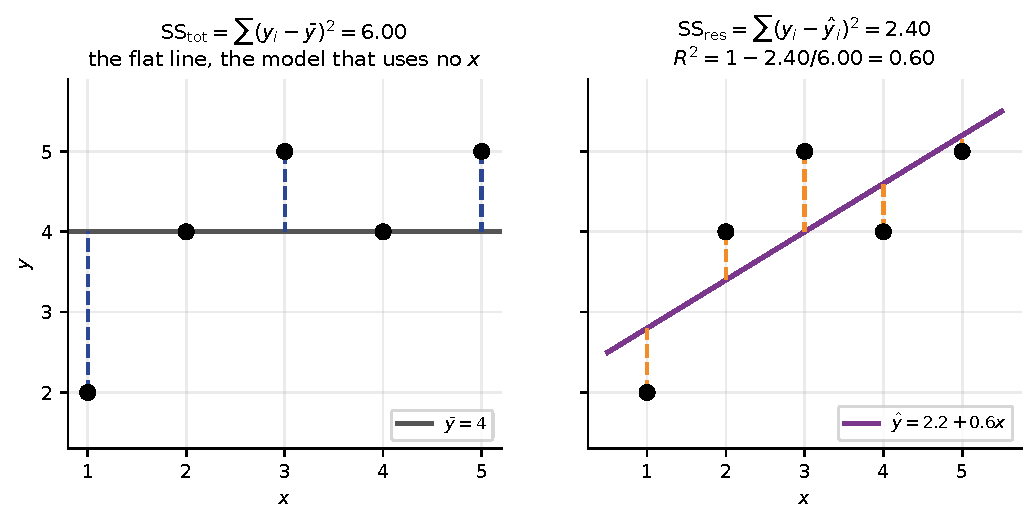
\includegraphics[width=0.86\textwidth]{r2hand.pdf}
  \end{center}
  \begin{center}\small
    Left, the dashed segments are the deviations from $\bar y = 4$: their
    squares add to $6.00$. Right, the deviations from the fitted line: their
    squares add to $2.40$. \textbf{$R^2$ is the fraction of the left picture
    that the right picture removed} --- $60\%$ of it.
  \end{center}
\end{frame}

\begin{frame}[fragile,shrink=6]{The same numbers from the library}
\begin{lstlisting}
from sklearn.metrics import r2_score
print(r2_score(y, yhat))                  # 1 - SSres/SStot
print(LinearRegression().fit(x[:, None], y).score(x[:, None], y))
\end{lstlisting}
\begin{outblk}
SSreg = SStot - SSres = 3.60      b1^2 * Sxx = 3.60
R2 = 1 - SSres/SStot = 1 - 2.40/6.00 = 0.6000
r^2 = (Sxy/sqrt(Sxx*Syy))^2 = 0.6000
sklearn r2_score            = 0.6000
s = sqrt(SSres/(n-2))       = 0.8944
\end{outblk}
\onslide<2->
\begin{center}\small
  Four routes to $0.6000$: the definition, the regression sum of squares, the
  squared correlation, and \texttt{r2\_score}. \textbf{\texttt{r2\_score} is
  three lines of arithmetic, not a verdict.} The next four slides are about
  what those three lines cannot see.
\end{center}
\end{frame}

\begin{frame}[fragile,shrink=8]{Predict first \#3}
$30$ rows. \textbf{One} real predictor, with $y = 1 + 2x + \varepsilon$ and a
noise sd of $2$. Its $R^2$ is $0.2413$.

Now append columns of $\mathcal{N}(0,1)$ \textbf{pure noise} --- generated
without ever looking at $y$ --- and refit, one column at a time, up to $27$
of them.

\begin{center}
  \textbf{What happens to $R^2$? Does it ever go down?}
\end{center}
\vspace{0.2em}
\onslide<2->
\begin{outblk}
  extra noise columns   p   R2        adjusted R2
         0             1   0.241296   +0.214199
         5             6   0.402777   +0.246979
        10            11   0.660344   +0.452777
        15            16   0.743023   +0.426743
        20            21   0.793909   +0.252920
        27            28   0.940085   -0.737539
R2 decreased at any step?  False   (28 nested models)
smallest single-step change +0.00000315
\end{outblk}
\onslide<3->
\begin{alertblock}{$0.2413 \rightarrow 0.9401$, and it never once fell}
  \footnotesize Not ``rarely fell'' --- \textbf{never}, across all $27$ steps,
  and the smallest step was $+4\times10^{-8}$, not $-4\times10^{-8}$. Adding a
  column can only enlarge the space of fits available, and the old fit is
  still in it (set the new coefficient to zero). \textbf{So $R^2$ is a
  monotone function of model size and cannot be used to choose one.}
\end{alertblock}
\end{frame}

\begin{frame}[fragile,shrink=8]{Adjusted $R^2$: a correction, and its limits}
  \[
    R^2_{\text{adj}} = 1 - (1 - R^2)\,\frac{n-1}{n-p-1}
  \]
  charges you $p$ degrees of freedom. On the $30$ rows it went
  $+0.2142 \rightarrow \mathbf{-0.7375}$: it caught the fraud completely.
  Now the same experiment on $442$ real patients:
\begin{outblk}
load_diabetes: 442 rows, 10 real features
  noise cols    p     R2        adjusted R2   5-fold CV R2
       0        10   0.517748   +0.506559     +0.489155
     100       110   0.643486   +0.525008     +0.337363
     200       210   0.759013   +0.539935     -0.105104
     400       410   0.976075   +0.659652     -5.760536
\end{outblk}
\onslide<2->
\begin{alertblock}{Adjusted $R^2$ was still saying $+0.54$ when the truth was $-8.83$}
  \footnotesize With $410$ junk columns on $442$ rows, $R^2 = 0.9761$ and
  \textbf{adjusted $R^2$ went \emph{up}, to $0.6597$}. Cross-validation said
  $-8.83$. \textbf{Adjusted $R^2$ is a penalty, not a test.} It is worth
  reporting and it is not worth trusting; the honest number is the one
  computed on rows the fit never saw.
\end{alertblock}
\end{frame}

\begin{frame}[shrink=8]{Drawn: the two curves that disagree}
  \begin{center}
    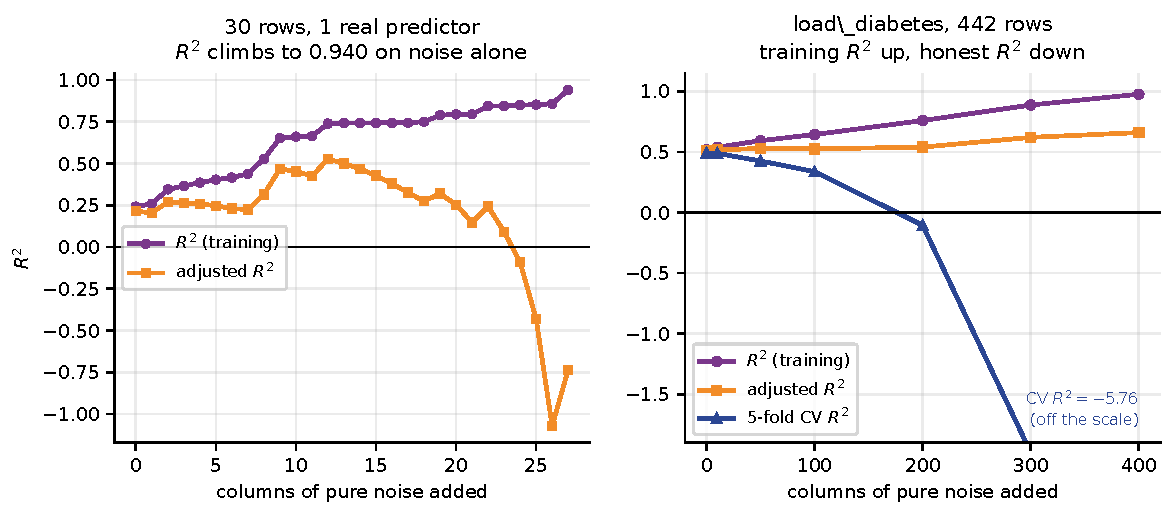
\includegraphics[width=0.94\textwidth]{r2noise.pdf}
  \end{center}
  \begin{center}\small
    Left, $30$ rows: $R^2$ climbs to $0.908$ on noise while adjusted $R^2$
    collapses. Right, $442$ rows: \textbf{$R^2$ climbs, adjusted $R^2$ stays
    flat and complacent near $0.5$, and cross-validated $R^2$ falls off the
    bottom of the chart.} Only the third curve is measuring prediction.
  \end{center}
\end{frame}

\begin{frame}[fragile,shrink=8]{Predict first \#4}
Three held-out points, $y_{\text{test}} = (1, 2, 3)$. Your model predicts
$(3, 2, 1)$ --- exactly backwards.

\begin{center}
  \textbf{What is $R^2$ on those three points? Is it allowed to be below
  zero?}
\end{center}
\vspace{0.2em}
\onslide<2->
\begin{outblk}
y_test       [1. 2. 3.]
prediction   [3. 2. 1.]
mean of y_test 2.0000  SStot 2.0000  SSres 8.0000
R2 = 1 - 8.0/2.0 = -3.0000     sklearn -3.0000
R2 of the constant prediction 2.0: 0.0000
\end{outblk}
\onslide<3->
\begin{alertblock}{$R^2 = -3$, and there is no lower bound at all}
  \footnotesize $R^2$ is only bounded below by $0$ \textbf{on the data the
  intercept was fitted to}, where $\bar y$ is available to the model for free.
  On \emph{held-out} rows $\bar y_{\text{test}}$ is a number the model never
  saw, so $\mathrm{SS_{res}}$ can exceed $\mathrm{SS_{tot}}$ without limit.
  \textbf{A negative held-out $R^2$ means: you would have done better
  predicting the mean and going home.}
\end{alertblock}
\end{frame}

\begin{frame}[shrink=8]{Drawn: negative $R^2$ on real held-out data}
  \begin{center}
    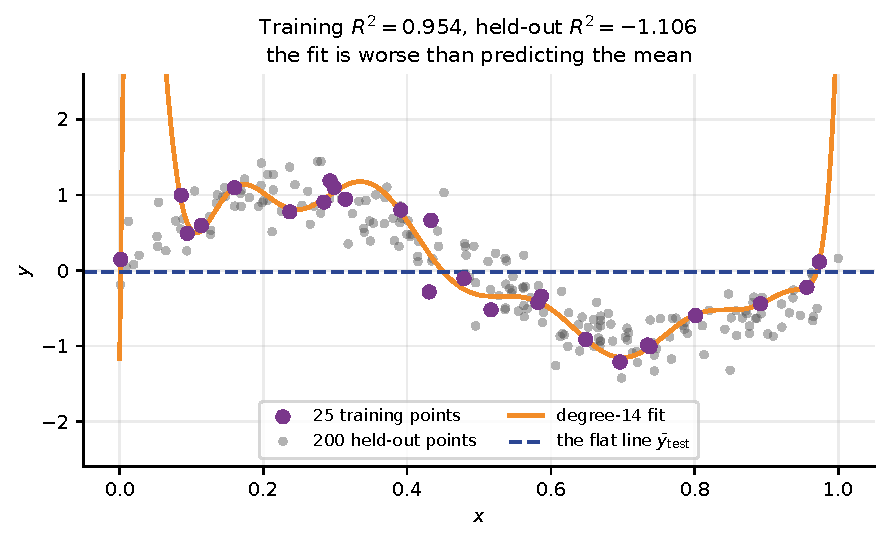
\includegraphics[width=0.72\textwidth]{r2negative.pdf}
  \end{center}
  \vspace{-0.2em}
  \begin{center}\small
    A degree-$14$ polynomial through $25$ training points: training
    $R^2 = 0.954$, held-out $R^2 = \mathbf{-1.106}$. The orange curve passes
    beautifully close to every purple point and leaves the data entirely
    between them. \textbf{The blue dashed line --- predict the mean, always
    --- beats it.}
  \end{center}
\end{frame}

% =====================================================================
\section[Adequacy]{Checking model adequacy}
\label{sec:adequacy}

\begin{frame}[shrink=6]{What one number cannot tell you}
  \begin{center}\small
  \begin{tabular}{@{}lp{7.6cm}@{}}
    \toprule
    \textbf{Assumption} & \textbf{What breaks it, and how you see it}\\
    \midrule
    \textbf{Linearity} & the truth bends. Residuals versus fitted show a
      systematic arch or U.\\[3pt]
    \textbf{Constant variance} & the spread grows with $\hat y$. The residual
      plot fans out.\\[3pt]
    \textbf{Normality} & heavy tails or skew. The normal Q--Q plot bends away
      from the line at the ends.\\[3pt]
    \textbf{Independence} & time or space structure. Residuals plotted in
      order drift or oscillate.\\[3pt]
    \textbf{No single point in charge} & one high-leverage row. Delete it and
      the slope moves.\\
    \bottomrule
  \end{tabular}
  \end{center}
  \vspace{0.3em}
  \begin{alertblock}{$R^2$ detects none of these}
    \small $R^2$ is a ratio of two sums. It cannot see the \emph{order} of the
    residuals, their \emph{shape}, or their \emph{pattern against $\hat y$}.
    \textbf{Four datasets are about to have the same $R^2$ and four completely
    different problems.}
  \end{alertblock}
\end{frame}

\begin{frame}[fragile,shrink=8]{Anscombe's quartet, computed}
Four datasets of eleven $(x,y)$ pairs, published by F.\ J.\ Anscombe in 1973.
You met them in L8; today we take the next step and read the residuals.
\begin{outblk}
set  mean x  mean y   sd x    sd y   intercept  slope    R2      SSres
I     9.000   7.501   3.317   2.032    3.0001  0.5001  0.6665  13.7627
II    9.000   7.501   3.317   2.032    3.0009  0.5000  0.6662  13.7763
III   9.000   7.500   3.317   2.030    3.0025  0.4997  0.6663  13.7562
IV    9.000   7.501   3.317   2.031    3.0017  0.4999  0.6667  13.7425
\end{outblk}
\onslide<2->
\begin{center}\small
  Same means to three decimals, same standard deviations, same fitted line
  $\hat y = 3.00 + 0.50x$, same $R^2 = 0.666$, same residual sum of squares to
  two decimals. \textbf{If you report the table above, you have told your
  reader that these four datasets are the same dataset.}
\end{center}
\onslide<3->
\begin{center}\small
  \textbf{They are not. Look at the next slide before you read the numbers
  again.}
\end{center}
\end{frame}

\begin{frame}[shrink=8]{Drawn: the four datasets}
  \begin{center}
    
\includegraphics[width=0.62\textwidth]{anscombe.pdf}
  \end{center}
  \vspace{-0.2em}
  \begin{center}\small
    \textbf{I} is a genuine noisy line. \textbf{II} is an exact parabola ---
    the wrong model, not noisy data. \textbf{III} is a perfect straight line
    with one contaminated point. \textbf{IV} has ten points at $x = 8$ and one
    at $x = 19$: \textbf{the eleventh point alone determines the slope}, and
    there is no evidence of linearity anywhere.
  \end{center}
\end{frame}

\begin{frame}[fragile,shrink=8]{The residual plot gives four different diagnoses}
  \begin{center}
    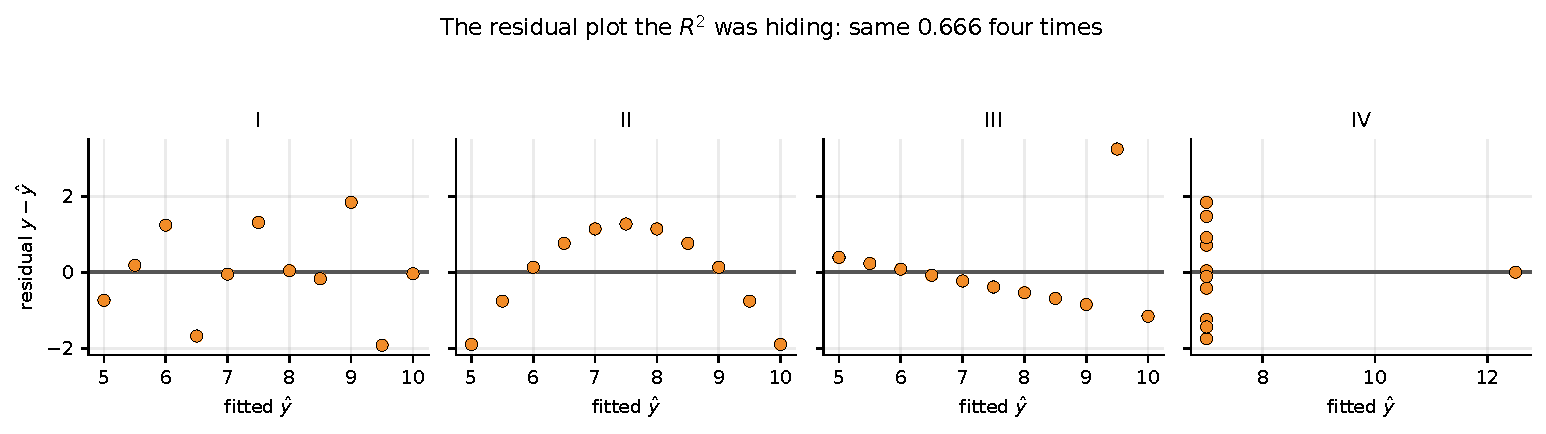
\includegraphics[width=0.90\textwidth]{ansresid.pdf}
  \end{center}
\begin{outblk}
set  max|e|  |e|max/|e|2nd  curvature R2  Shapiro p  max leverage  slope w/o pt
I     1.921           1.04        0.0623     0.5456        0.3182        0.5028
II    1.901           1.00        1.0000     0.0929        0.3182        0.6267
III   3.241           2.80        0.0550     0.0016        0.3182        0.5770
IV    1.839           1.05        0.0000     0.7800        1.0000     undefined
\end{outblk}
\onslide<2->
\begin{center}\footnotesize
  \textbf{II}: a parabola fitted to the residuals explains
  $\mathbf{100.00\%}$ of them --- there is no noise left, only unmodelled
  curvature. \textbf{III}: the largest residual is $2.80\times$ the next, and
  Shapiro rejects normality at $p = 0.0016$. \textbf{IV}: leverage
  $\mathbf{1.0000}$, and deleting that one row leaves the slope
  \textbf{undefined}. Same $R^2$, four different failures.
\end{center}
\end{frame}

\begin{frame}[fragile,shrink=8]{Non-constant variance, measured}
$200$ points, $y = 3 + 2x + x\varepsilon/4$: the noise grows with $x$.
\begin{outblk}
fit: intercept 2.8790  slope 2.0011   R2 0.9267
residual sd, lower half of x  1.0460
residual sd, upper half of x  1.8988   ratio 1.82
Breusch-Pagan LM = n*R2(e^2 on yhat) = 22.9065   chi2(1) p = 0.000002
Shapiro-Wilk on the residuals p = 0.031073
after log(y): Breusch-Pagan LM = 3.2426   p = 0.0717   sd ratio 0.89
\end{outblk}
\onslide<2->
\begin{alertblock}{$R^2 = 0.9267$ and the model is wrong anyway}
  \footnotesize The coefficients are still unbiased --- least squares does not
  need constant variance for that. What breaks is everything
  \emph{downstream}: standard errors, $p$-values, confidence intervals and
  prediction intervals are all computed as if $\sigma$ were one number, and it
  is not. \textbf{$\log y$ takes it most of the way back: the test statistic
  falls from $22.91$ to $3.24$, $p$ from $2\times10^{-6}$ to $0.072$} --- an
  improvement, not a cure.
\end{alertblock}
\end{frame}

\begin{frame}[shrink=8]{Drawn: the fan, and what a transform does to it}
  \begin{center}
    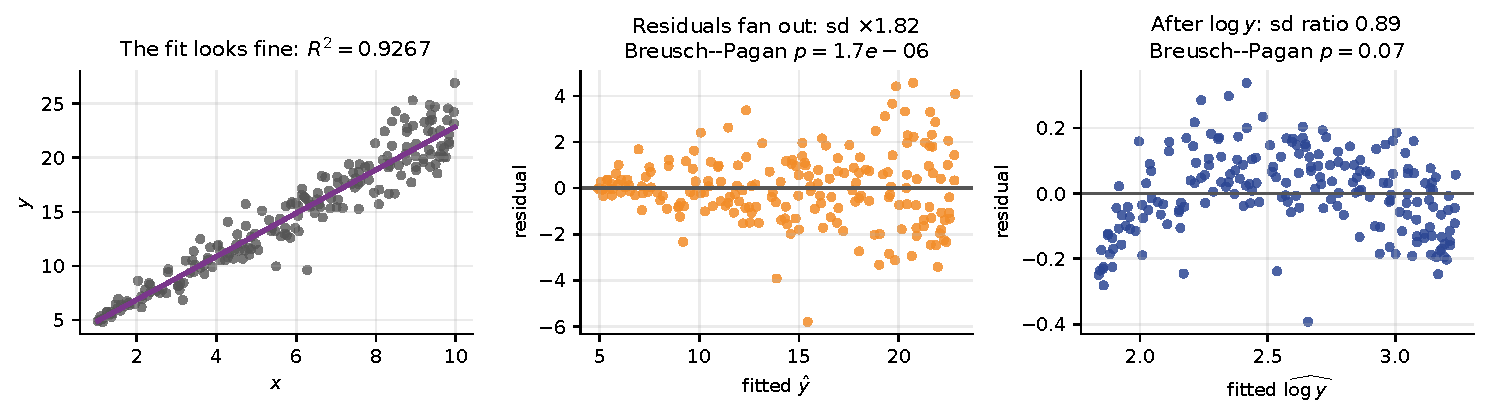
\includegraphics[width=0.96\textwidth]{hetero.pdf}
  \end{center}
  \begin{center}\small
    The left panel is the one you would put in a report. The middle panel is
    the one that tells you the truth --- the residual cloud is a wedge, wide
    on the right. The right panel is the same data after $\log y$:
    \textbf{a shapeless band, which is what a residual plot should look like.}
  \end{center}
\end{frame}

\begin{frame}[fragile,shrink=8]{The normal Q--Q plot, and how to read it}
Sort the residuals; plot them against the normal quantiles they would occupy
if they were Gaussian. Straight line, Gaussian residuals.
\begin{outblk}
residual model     corr(ordered resid, normal quantile)   Shapiro p   kurtosis
Gaussian noise                              0.9935    0.198668    -0.5004
t(3) noise                                  0.9626    0.000009     2.7920
uniform noise                               0.9845    0.003336    -1.0901
\end{outblk}
\onslide<2->
\begin{center}
  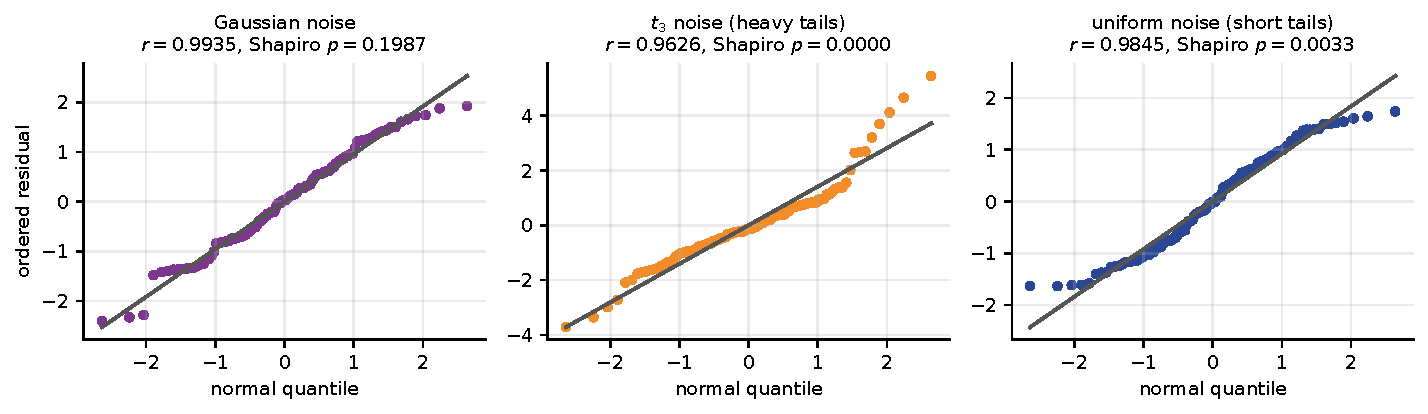
\includegraphics[width=0.86\textwidth]{qqplots.pdf}
\end{center}
\onslide<3->
\begin{center}\footnotesize
  \textbf{All three correlations are above $0.97$} --- the eyeball is far more
  discriminating here than the summary statistic. $t_3$ bends \emph{away} from
  the line at both ends (heavy tails); uniform bends \emph{towards} it (short
  tails). Neither is fatal for the coefficients; both invalidate the
  $p$-values.
\end{center}
\end{frame}

% =====================================================================
\section[Over-fitting]{Over-fitting and its detection}
\label{sec:overfit}

\begin{frame}[shrink=6]{Over-fitting, defined by two error curves}
  \begin{exampleblock}{}
    \centering
    A model \textbf{over-fits} when it is learning the noise in the training
    rows --- structure that will not repeat.
  \end{exampleblock}
  \vspace{0.2em}
  \begin{columns}[T]
    \begin{column}{0.48\textwidth}
      \begin{block}{The signature}
        \small Training error keeps falling. Error on rows the model has never
        seen \textbf{stops falling and turns up}. The gap between the two is
        the amount of noise memorised.
      \end{block}
    \end{column}
    \begin{column}{0.48\textwidth}
      \begin{alertblock}{Why it must happen}
        \small A degree-$d$ polynomial through $n$ points has $d+1$ free
        parameters. At $d + 1 = n$ it passes through \emph{every} point
        exactly, noise included, and $R^2 = 1$. \textbf{Perfect training fit
        is a symptom, not an achievement.}
      \end{alertblock}
    \end{column}
  \end{columns}
  \vspace{0.2em}
  \begin{center}\small
    The running example: $25$ points from $y = \sin 2\pi x + \varepsilon$ with
    $\sigma = 0.25$. \textbf{We know the truth and the noise floor, which is
    why this example can be graded.}
  \end{center}
\end{frame}

\begin{frame}[shrink=8]{Drawn: the same 25 points, four models}
  \begin{center}
    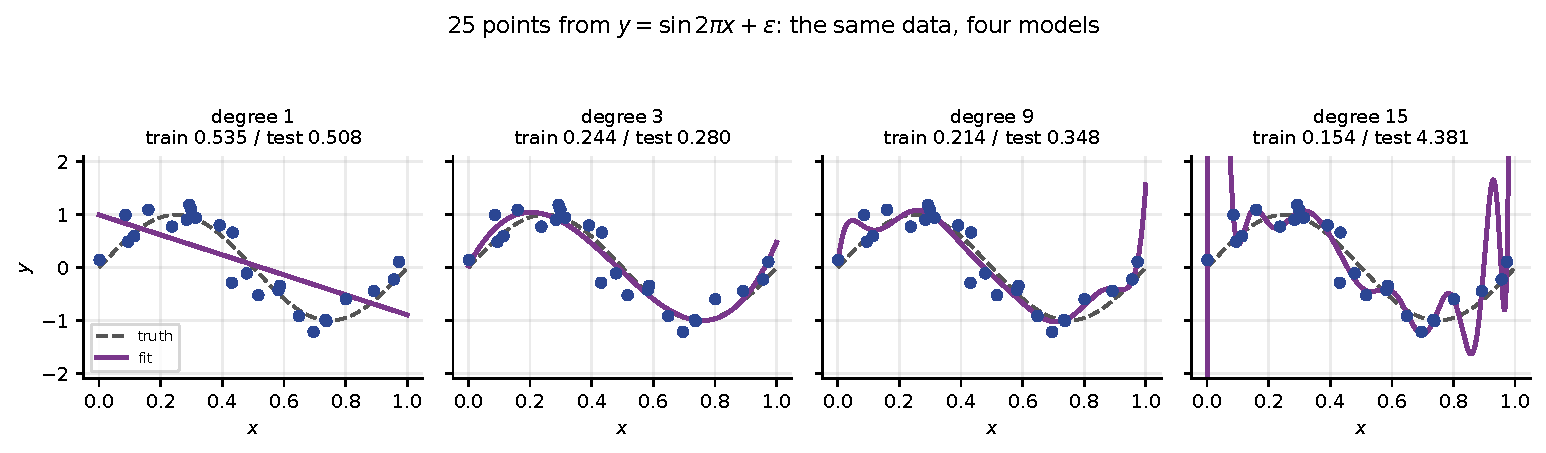
\includegraphics[width=0.98\textwidth]{polyfits.pdf}
  \end{center}
  \begin{center}\small
    Degree $1$ cannot bend at all --- \textbf{under-fitting}, and both errors
    are large. Degree $3$ tracks the truth. Degree $9$ has started to ripple.
    Degree $15$ passes near every point and \textbf{leaves the dashed truth
    entirely}: train $0.154$, test $4.381$.
  \end{center}
\end{frame}

\begin{frame}[fragile,shrink=8]{Predict first \#5}
Fit polynomials of degree $0$ to $20$ to those $25$ points. Score each on the
training rows and on $2000$ fresh rows from the same generator.

\begin{center}
  \textbf{At which degree does the test error stop improving? And how bad does
  degree $20$ get?}
\end{center}
\vspace{0.2em}
\onslide<2->
\begin{outblk}
degree  params  train RMSE   test RMSE
   1       2      0.5347        0.5084
   3       4      0.2441        0.2795   <-- test minimum
   5       6      0.2273        0.2828
   9      10      0.2143        0.3484
  12      13      0.1843        0.5966
  15      16      0.1540        4.3811
  20      21      0.1466      153.1554
train RMSE strictly non-increasing? True   largest increase -3.29e-05
test minimum at degree 3, RMSE 0.2795   (noise floor 0.2500)
\end{outblk}
\onslide<3->
\begin{alertblock}{The turn is at degree \textbf{3}, and degree 20 is $\mathbf{548\times}$ worse}
  \footnotesize Train RMSE fell at \emph{every one} of the twenty steps ---
  verified, not asserted --- from $0.7507$ to $0.1466$. Test RMSE bottomed at
  $0.2795$, a whisker above the noise floor of $0.2500$, and then went to
  $153$. \textbf{Between degree 3 and degree 20 the training score improved by
  $40\%$ and the model became unusable.}
\end{alertblock}
\end{frame}

\begin{frame}[shrink=8]{Drawn: the two curves that define over-fitting}
  \begin{center}
    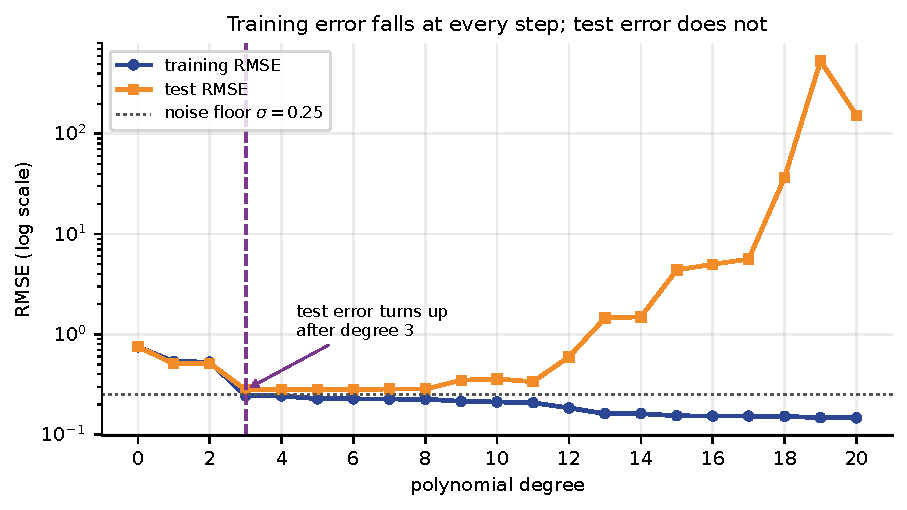
\includegraphics[width=0.72\textwidth]{overfit.pdf}
  \end{center}
  \vspace{-0.2em}
  \begin{center}\small
    Log scale on the vertical axis, or the right-hand end would not fit on the
    page. \textbf{The blue curve is monotone by construction} --- a
    degree-$(d{+}1)$ model contains every degree-$d$ model. The orange curve
    owes you nothing, and after degree $3$ it stops paying.
  \end{center}
\end{frame}

\begin{frame}[fragile,shrink=8]{More rows move the turning point}
The same generator, the same degrees, only $n_{\text{train}}$ changes.
\begin{outblk}
 n_train   best degree   test RMSE at best   test RMSE at degree 20
     15         3              0.2959               13292.3268
     25         5              0.3102                2867.4761
     50         6              0.2634                   0.3256
    200         5              0.2547                   0.2656
   1000         7              0.2536                   0.2572
\end{outblk}
\onslide<2->
\begin{alertblock}{At $n = 1000$, degree $20$ costs almost nothing}
  \footnotesize $0.2572$ against a best of $0.2536$ and a noise floor of
  $0.2500$. The \emph{same} twenty-one-parameter model that was catastrophic
  on $15$ rows is harmless on $1000$. \textbf{Over-fitting is not a property
  of the model. It is a property of the model \emph{and} the amount of data
  you have} --- which is why ``how complex a model may I use?'' has no answer
  until you say $n$.
\end{alertblock}
\end{frame}

\begin{frame}[fragile,shrink=8]{And it happens on real data, not just sine waves}
\texttt{load\_diabetes}, $442$ patients, split $75/25$. Add polynomial
interactions of the ten features.
\begin{outblk}
model                          train R2    5-fold CV R2   held-out R2   params
linear (10 features)         +0.5554        +0.5224        +0.3594          10
degree-2 polynomial          +0.6469        +0.3827        +0.2440          65
degree-3 polynomial          +0.9179     -1212.1828       -22.0428         285
predicting the training mean for every patient: held-out R2 -0.0001
\end{outblk}
\onslide<2->
\begin{alertblock}{Training $R^2$ of $0.92$, held-out $R^2$ of $-22$}
  \footnotesize $285$ parameters and $331$ training rows. The training column
  goes \textbf{up} at every row of the table and the held-out column goes
  \textbf{down} at every row. \textbf{Reading only the training column, you
  would ship the worst of the three.} And the last line is the yardstick: even
  predicting a constant beats $-22$.
\end{alertblock}
\end{frame}

% =====================================================================
\section[CV]{Cross-validation as the detector}
\label{sec:cv}

\begin{frame}[shrink=6]{The idea, in three sentences}
  \begin{block}{$k$-fold cross-validation --- the mechanism from Unit IV}
    \small Split the training rows into $k$ equal parts. For each part in
    turn: fit on the other $k-1$ parts, score on the held-out part. Average
    the $k$ scores.
  \end{block}
  \vspace{0.2em}
  \begin{columns}[T]
    \begin{column}{0.48\textwidth}
      \begin{exampleblock}{What it buys}
        \small Every row is used for testing exactly once and for training
        $k-1$ times. \textbf{You get a held-out estimate without spending a
        held-out set}, and you get $k$ of them, so you get a spread too.
      \end{exampleblock}
    \end{column}
    \begin{column}{0.48\textwidth}
      \begin{alertblock}{What it costs}
        \small $k$ model fits instead of one. And \textbf{LOOCV}, the case
        $k = n$, costs $n$ fits --- but has no split lottery at all, because
        there is only one way to leave one out.
      \end{alertblock}
    \end{column}
  \end{columns}
  \vspace{0.2em}
  \begin{center}\small
    The test set is \textbf{not} part of this. It is opened once, at the end,
    to report a number --- never to choose a degree.
  \end{center}
\end{frame}

\begin{frame}[fragile,shrink=8]{The detector, run on the over-fitting example}
\begin{lstlisting}
pipe = make_pipeline(PolynomialFeatures(d), LinearRegression())
cv = -cross_val_score(pipe, x[:, None], y, cv=KFold(5, shuffle=True,
                      random_state=0), scoring="neg_root_mean_squared_error")
\end{lstlisting}
\begin{outblk}
degree   train RMSE   5-fold CV RMSE   LOOCV RMSE     test RMSE
   1      0.5347          0.6319        0.5895        0.5084
   3      0.2441          0.3239        0.2799        0.2795
   5      0.2273          0.6711        0.2912        0.2828
   9      0.2143         32.7952        0.4516        0.3484
  15      0.1540      23379.8414       49.8944        4.3811
train RMSE picks degree 15 (the largest offered)   5-fold CV picks degree 3
LOOCV      picks degree 3                          the test set says       3
\end{outblk}
\onslide<2->
\begin{alertblock}{Three of the four columns agree, and it is the wrong one that differs}
  \footnotesize Train RMSE picks the biggest model on offer, as it always
  will. \textbf{5-fold CV and LOOCV both pick degree $3$ --- the same answer
  the test set gives --- using nothing but the $25$ training rows.} That is
  the whole argument for cross-validation in one table.
\end{alertblock}
\end{frame}

\begin{frame}[shrink=8]{Drawn: four curves, one of them unavailable}
  \begin{center}
    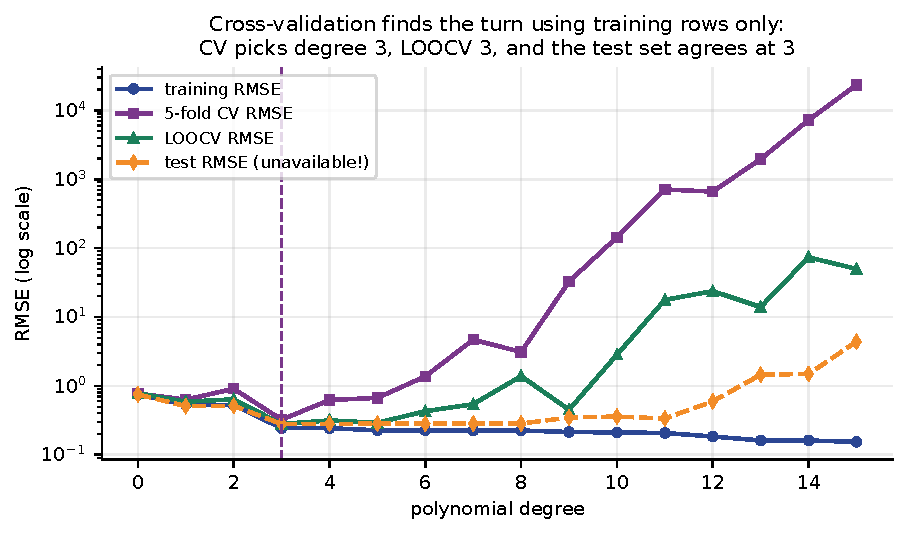
\includegraphics[width=0.72\textwidth]{cvdetect.pdf}
  \end{center}
  \vspace{-0.2em}
  \begin{center}\small
    The orange dashed curve is the test error --- drawn here only because this
    is a demonstration; \textbf{in a real project you may not look at it}. The
    purple and green curves reproduce its minimum without it. LOOCV tracks the
    test curve more closely at small degree; 5-fold is noisier and $3\times$
    cheaper here, $5\times$ against $25$ fits.
  \end{center}
\end{frame}

\begin{frame}[fragile,shrink=8]{Why not just hold out one validation set?}
Split the same $25$ rows $60/40$, ten different ways, and let each split
choose the degree.
\begin{outblk}
ten different single validation splits of the same 25 rows
  degree chosen by each split: [3, 3, 3, 3, 4, 5, 3, 3, 3, 3]
  chosen degrees range from 3 to 5
  spread of the estimated RMSE at degree 3: 0.2243 to 0.4415
5-fold CV RMSE at degree 3 (one number, no split lottery): 0.3239
\end{outblk}
\onslide<2->
\begin{center}
  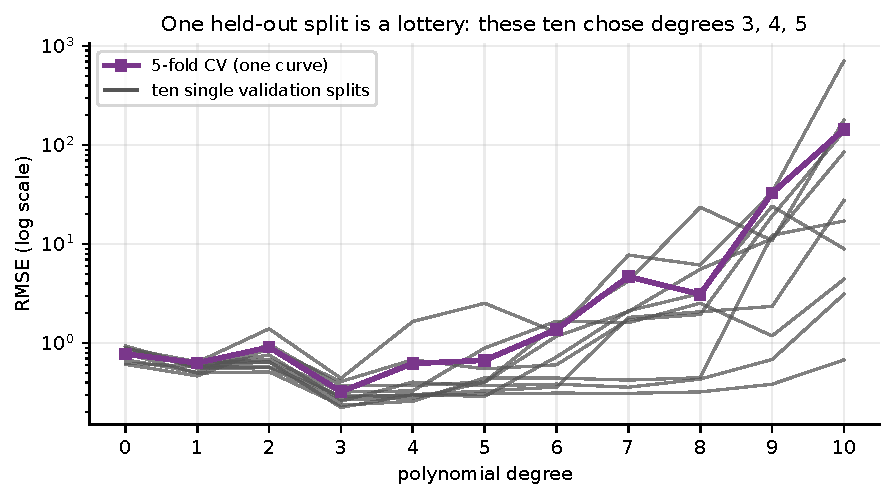
\includegraphics[width=0.62\textwidth]{valsplit.pdf}
\end{center}
\onslide<3->
\begin{center}\footnotesize
  Seven of the ten splits chose degree $3$ and three did not --- and the
  \emph{estimate} of the error at degree 3 ranged from $0.2243$ to $0.4415$,
  \textbf{a factor of two, from nothing but which rows landed in which half}.
  $k$-fold averages that lottery away and uses every row.
\end{center}
\end{frame}

\begin{frame}[shrink=6]{Choosing $k$, and the rule that outranks it}
  \begin{center}\small
  \begin{tabular}{@{}lp{3.5cm}p{3.5cm}@{}}
    \toprule
    & \textbf{Bias of the estimate} & \textbf{Variance / cost}\\
    \midrule
    $k = 2$ & pessimistic: each fit sees half the data & cheap, but noisy\\[3pt]
    $k = 5$ or $10$ & small; the usual choice & moderate, $5$--$10$ fits\\[3pt]
    $k = n$ (LOOCV) & almost none: each fit sees $n-1$ rows & $n$ fits;
      the folds overlap heavily\\
    \bottomrule
  \end{tabular}
  \end{center}
  \vspace{0.3em}
  \begin{alertblock}{The rule that matters more than $k$}
    \small \textbf{Everything the model learns must be refitted inside every
    fold.} A degree, a scaler, a feature selection, a threshold. If a choice
    was made using all the rows and then cross-validated, the score is not a
    held-out score --- as the splitting and validation lecture measured, and
    as Unit VI will measure again.
  \end{alertblock}
  \vspace{0.1em}
  \begin{center}\small
    \texttt{Pipeline} exists precisely so that this is the easy thing to do.
  \end{center}
\end{frame}

% =====================================================================
\section{Summary}
\label{sec:summary}

\begin{frame}[shrink=16]{Summary --- twelve lines}
  \begin{enumerate}\small
    \item ``Closest'' is a choice. On five points the direct slope is
      $0.6000$, the inverse slope $1.0000$, the orthogonal slope $0.7208$; the
      ratio of the first two is $r^2 = 0.6$. Each wins only its own criterion.
    \item \textbf{Assume $\varepsilon_i \sim \mathcal{N}(0,\sigma^2)$ i.i.d.,
      take logs, and the log-likelihood is
      $\text{const} - \mathrm{SSE}/(2\sigma^2)$. Maximising it is exactly
      minimising the SSE.} Least squares is the Gaussian MLE.
    \item $\sigma^2$ does not move the estimate: the same $b_1 = 0.60000$
      maximised the likelihood at $\sigma^2 = 0.48$ and at $\sigma^2 = 1$.
    \item $\hat\sigma^2_{\mathrm{ML}} = \mathrm{SSE}/n$ is \textbf{biased
      downwards} by $(n-2)/n$. Over $20{,}000$ datasets with $\sigma^2 = 4$ and
      $n = 10$ it averaged $3.2117$ against a predicted $3.2000$, and was too
      small in $73.4\%$ of runs. Use $s^2 = \mathrm{SSE}/(n-2)$.
    \item Change the noise to Laplace and the MLE becomes least
      \emph{absolute} deviations. Each estimator won its own criterion.
    \item $R^2 = 1 - \mathrm{SS_{res}}/\mathrm{SS_{tot}} = 1 - 2.40/6.00 =
      0.6000$ on the five points, equal to $r^2$ and to $b_1^2S_{xx}/
      \mathrm{SS_{tot}}$.
    \item \textbf{$R^2$ never falls when you add a column.} $27$ pure-noise
      columns on $30$ rows took it from $0.2413$ to $0.9401$, never once
      decreasing.
    \item Adjusted $R^2$ caught that ($-0.7375$) but on $442$ rows with $410$
      junk columns it read $+0.6597$ while cross-validation read $-5.7605$.
      A penalty, not a test.
    \item Held-out $R^2$ has \textbf{no lower bound}: $-3$ on three points by
      hand, $-1.106$ for a degree-14 fit, $-22.04$ on diabetes.
    \item Anscombe's four datasets share every summary statistic and
      $R^2 = 0.666$. The residual plot separates them: curvature $R^2 = 1.0000$
      for II, largest residual $2.80\times$ the next for III, leverage
      $1.0000$ for IV.
    \item Over-fitting: train RMSE fell at all $20$ steps, test RMSE turned up
      after \textbf{degree 3} and reached $153$ at degree 20 --- $548\times$
      worse. At $n = 1000$ the same degree 20 costs $0.0036$.
    \item \textbf{5-fold CV and LOOCV both picked degree 3, the same answer as
      the test set, using only the training rows.} One held-out split picked
      3, 4 or 5 depending on the seed.
  \end{enumerate}
\end{frame}

\begin{frame}[shrink=3]{Before the next lecture}
  \begin{columns}[T]
    \begin{column}{0.48\textwidth}
      \begin{block}{Read}
        \texttt{notes.pdf} --- the maximum likelihood derivation written out
        line by line, the proof that $\mathbb{E}[\mathrm{SSE}] =
        (n-2)\sigma^2$, and \textbf{10 practice questions with full worked
        solutions}.
      \end{block}
      \begin{block}{Do}
        Questions 2, 4 and 7. Question 2 is the derivation from a blank page;
        question 4 is $R^2$ by hand; question 7 is a debugging story you will
        meet for real.
      \end{block}
    \end{column}
    \begin{column}{0.48\textwidth}
      \begin{exampleblock}{Next: logistic regression}
        The response becomes a class label. \textbf{Carry the method, not the
        formula}: write the likelihood, take logs, maximise. Squares will not
        appear --- because the noise is no longer Gaussian.
      \end{exampleblock}
      \begin{alertblock}{And a habit to start now}
        Never report an $R^2$ without a residual plot beside it, and never
        report a training score as if it were a result.
      \end{alertblock}
    \end{column}
  \end{columns}
  \begin{center}
    \small Materials: \texttt{\AMLRepoURL}
  \end{center}
  \slidesources{\AMLUnitVSources}
\end{frame}

\end{document}
